\documentclass{beamer}

% === AUTOR === (((
\author{\textit{Por Erick I. Rodríguez Juárez.}}
% )))

% === PAQUETES === (((
% \usepackage{makeidx}
% \usepackage{xltxtra}
\usepackage{amsfonts}
\usepackage{amsmath}
\usepackage{amssymb}
% \usepackage{fullpage}
\usepackage{tikz}
\usetikzlibrary{arrows.meta}
\usepackage{graphicx}
% )))

% === TIPOGRAFÍA === (((
% \setmainfont[
  % BoldFont       = bodonibi,
	% ItalicFont     = Century modern italic2.ttf,
	% BoldItalicFont = bodonibi,
	% SmallCapsFont  = lmromancaps10-regular.otf
% ]{Century_modern.ttf}
% )))

% === COMANDOS === (((
% \newcommand{\dis}{\displaystyle}
% \newcommand{\qed}{\hspace{0.5cm}\rule{0.16cm}{0.4cm}}
% \newcommand{\operator}[1]{\mathop{\vphantom{\sum}\mathchoice
% {\vcenter{\hbox{\huge $#1$}}}
% {\vcenter{\hbox{\Large $#1$}}}{#1}{#1}}\displaylimits}
% \newcommand{\suma}{\operator{
\includegraphics[scale=0.09]{FOTOS/Sigma.png}}}
% \setlength{\parindent}{0mm}
% )))

% === ITALICA EN ENTORNO MATEMÁTICO === (((
% \DeclareSymbolFont{italics}{\encodingdefault}{\rmdefault}{m}{it}
% \DeclareSymbolFontAlphabet{\mathit}{italics}
% \ExplSyntaxOn
% \int_step_inline:nnnn { `A } { 1 } { `Z }
 % {  \exp_args:Nf \DeclareMathSymbol{\char_generate:nn{#1}{11}}{\mathalpha}{italics}{#1} }
% \int_step_inline:nnnn { `a } { 1 } { `z } {  \exp_args:Nf \DeclareMathSymbol{\char_generate:nn{#1}{11}}{\mathalpha}{italics}{#1}}
% \ExplSyntaxOff
% )))

\begin{document}

\frame{\titlepage}

\begin{frame}[t]
	\frametitle{Teorema de Existencia y Unicidad.}
\begin{block}{Teorema de Existencia y Unicidad.}
	Considere el P.V.I. siguiente
	\[
		a_n(x) y^{(n)} + a_{n-1} (x) y^{(n-1)} + \;\cdots\; + a_1(x) y' +a_0(x) y = g(x).
	\]
	Sujeto a \(a_n(x) , a_{n-1} (x) , \;\cdots\; a_1(x) ,a_0(x)\) y \(g(x)\) continuas en el intervalo \(I\) y además, \(a_n(x) \ne 0\), \(\forall x \in I\). Si \(x=x_0\) en cualquier punto en el intervalo \(I\), entonces existe una única solución para el P.V.I. en \(I\).
\end{block}
	\begin{example}
		Determina si el P.V.I. \(x^2y'' -2xy' +2y=6\), \(y(0) =3\), \(y' (0) =1\), para \(x \in (- \infty , \infty)\) tiene solución única usando e T.E. y U.
	\end{example}
\end{frame}
\begin{frame}[t]
	\begin{exampleblock}{}
		\textbf{Solución.} Sean \(a_2(x) = x^2\), \(a_1(x) = -2x\), \(a_0(x) = 2\), \(g(x) = 6\) funciones continuas en el intervalo \((- \infty , \infty)\). \\[2mm]
		Pero
		\[
			\begin{array}{rcl}
				a_2(x) & = & x^2 = 0 \iff x = 0 \\[2mm]
				a_2(x) & = & x^2 \ne 0 \mbox{ en } (- \infty ,0) \mbox{ o } (0, \infty) \mbox{ pero éstos intervalos} \\[2mm]
				&& \mbox{no contienen a } x=0. \\[2mm]
				\therefore && \mbox{no se garantiza la existencia y unicidad de la} \\[2mm]
				&& \mbox{solución del P.V.I.}
			\end{array}
		\]
		Verifiquemos que \(y(x) = cx^2+x+3\) es solución del P.V.I. \(\forall c\). \\[2mm]
		Derivando:
		\[
			\begin{array}{rcl}
				y\,' & = & 2cx+1 \\[2mm]
				y\,'' & = & 2c.
			\end{array}
		\]
	\end{exampleblock}
\end{frame}

\begin{frame}[t]
	\begin{exampleblock}{}
		Sustiyuendo \(y\), \(y\,'\), \(y\,''\) en la E.D
		\[
			\begin{array}{rcl}
				x^2(2c) -2x(2cx+1) +2(c^2+x+3) & = & 6 \\[2mm]
				\iff \cancel{2cx^2} - \cancel{4cx^2} - \cancel{2x} + \cancel{2cx^2} + \cancel{2x} + 6 & = & 6 \\[2mm]
				6 & = & 6. \hspace{5mm}\forall c.
			\end{array}
		\]
		Veamos si \(y(x)\) satisface las C.I. \(y(0) =3\) y \(y\,' (0) =1\),
		\[
			\begin{array}{rcl}
				y(0) = c(0)^2+0+3 & = & 3 \\[2mm]
				3 & = & 3. \\[2mm]
				y\,' (0) = 2c(0) +1 & = & 1 \\[2mm]
				1 & = & 1.
			\end{array} \hspace{1cm} \forall c.
		\]
	\end{exampleblock}
\end{frame}

\begin{frame}[t]
	\begin{exampleblock}{}
		\begin{figure}[hbt!]
			\centering
			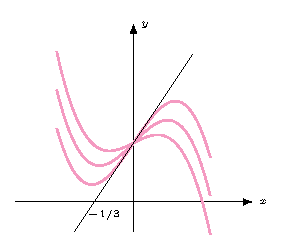
\includegraphics[width= 0.7 \linewidth]{IMAGENES/6/tikz.pdf}
		\end{figure}
		Al igual que los P.V.I., los P.V.F. pueden tener muchas soluciones, sólo una, o ninguna.
	\end{exampleblock}
\end{frame}

\begin{frame}[t]
	\begin{example}
		Considere la E.D. \(x'' +16x=0\), y \(x(t) = c_1 \cos 4t+c_2 \sin 4t\), la solución general explícita de dicha E.D.
		Encuentra la solución del problema de valor en la frontera cuyas condiciones son:
		\begin{enumerate}
			\item \(x(0) =0\), \(x(\pi /2) =0\).
			\item \(x(0) =0\), \(x(\pi /2) =1\).
			\item \(x(0) =0\), \(x(\pi /8) =0\).
		\end{enumerate}
		\textbf{Solución.} 
		\begin{enumerate}
			\item Apliquemos la C.F. en la solución general
		\[
			\begin{array}{rcl}
				x(0) = c_1 \cancelto{1}{\cos 4(0)} +c_2 \cancelto{0}{\sin 4(0)} & = & 0 \\[2mm]
				\iff c_1 & = & 0.\\[2mm]
				x(\pi /2) = c_1 \cos (4 \pi /2) + c_2 \sin (4 \pi /2) & = & 0 \\[2mm]
				\iff c_1 \cancelto{1}{\cos (2 \pi)} + c_2 \cancelto{0}{\sin (2 \pi)} & = & 0 \\[2mm]
				\iff c_1 & = & 0. \hspace{1cm} c_2 \in \mathbb{R}.
			\end{array}
		\]
		\end{enumerate}
	\end{example}
\end{frame}

\begin{frame}[t]
	\begin{exampleblock}{}
		\(\therefore \hspace{5mm} x(t) = c_2 \sin 4t\) es una familia de soluciones que satisfacen el P.V.F. Es decir, hay un número infinito de soluciones.
		\begin{figure}[hbtp!]
			\centering
			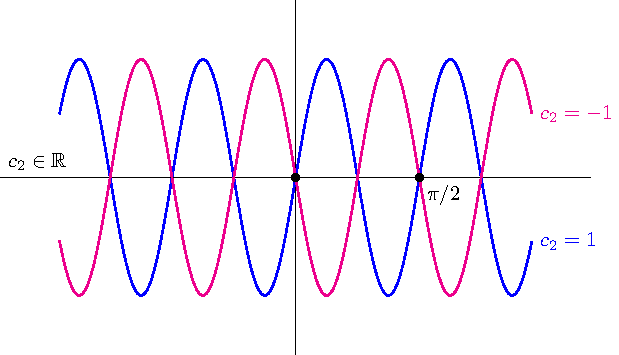
\includegraphics[width= 0.5 \linewidth]{IMAGENES/7/tikz.pdf}
		\end{figure}
		\begin{enumerate}
			\setcounter{enumi}{1}
		\item \vspace{-5mm}
			\[
				\begin{array}{rcl}
					x(0) = c_1 \cancelto{1}{\cos 4(0)} + c_2 \cancelto{0}{\sin 4(0)} & = & 0 \\[2mm]
					\iff c_1 & = & 0.\\[2mm]
					x(\pi /2) = c_1 \cos (4 \pi /2) + c_2 \sin (4 \pi /2) & = & 1 \\[2mm]
					\iff c_1 \cancelto{1}{\cos (2 \pi)} + c_2 \cancelto{0}{\sin (2 \pi)} & = & 1 \\[2mm]
					c_1 & = & 1.
				\end{array}
			\]
		\end{enumerate}
	\end{exampleblock}
\end{frame}

\begin{frame}[t]
	\begin{exampleblock}{}
		\begin{enumerate}
			\setcounter{enumi}{2}
		\item Aplicando las condiciones \(x(0) = 0\), \(x(\pi /8) =0\),
			\[
				\begin{array}{rcl}
					x(0) = c_1 \cancelto{1}{\cos 4(0)} + c_2 \cancelto{0}{\sin 4(0)} & = & 0 \\[2mm]
					\iff c_1 & = & 0. \\[2mm]
					x(\pi /8) = c_1 \cancelto{0}{\cos (4 \pi /8)} + c_2 \cancelto{1}{\sin (4 \pi /8)} & = & 0 \\[2mm]
					\iff c_2 & = & 0. \\[2mm]
					\therefore \hspace{5mm} x(t) & = & 0.
				\end{array}
			\]
				\begin{figure}[hbtp!]
					\centering
					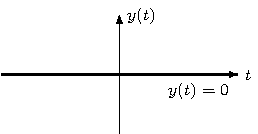
\includegraphics[width= 0.6 \linewidth]{IMAGENES/8/tikz.pdf}
				\end{figure}
		\end{enumerate}
	\end{exampleblock}
\end{frame}

\end{document}
